\section{Experiments}
In this section we demostrate the capabilities of \frameworkname~using four case studies. We selected as representative input application a matrix vector multiplication having dimension 5x5,10x10 and 15x15 and a matrix matrix multiplication having dimensions 10x10.
In our experiments we analyse the architectures generated by \frameworkname~and we derive the energy consumption and latency of each design. We use the information contained in the input \textit{Configuration Parameters} - \ref{ssec:conf_param} - to derive the dynamic and static energy consumed by each FU. Each generated architecture has a known latency imposed in each iteration of the DSE(\ref{ssec:dse}), which we use to compute its static energy consumption. Moreover, after applying the Modified Interval Partitioning algorithm (see~\ref{ssec:modified_interval_partitioning}), the instructions performed by each FU are known and this information is used to compute the dynamic energy consumption of an architecture.
In the first experiment - \ref{ssec:exp_single} - we show the result of the DSE methodology presented in section~\ref{ssec:dse}. The second experiments compares the use of MRAM memory - modeled according to~\cite{8310393} - at the Level 2 memory against the use of SRAM - TSMC tt0p9v85c for the two input applications. The last experiment compares different matrix dimensions for the Matrix Vector application, 5x5, 10x10 and 15x15.


\subsection{Single SRAM configuration}
\label{ssec:exp_single}

\begin{figure}[tb] 
\centering
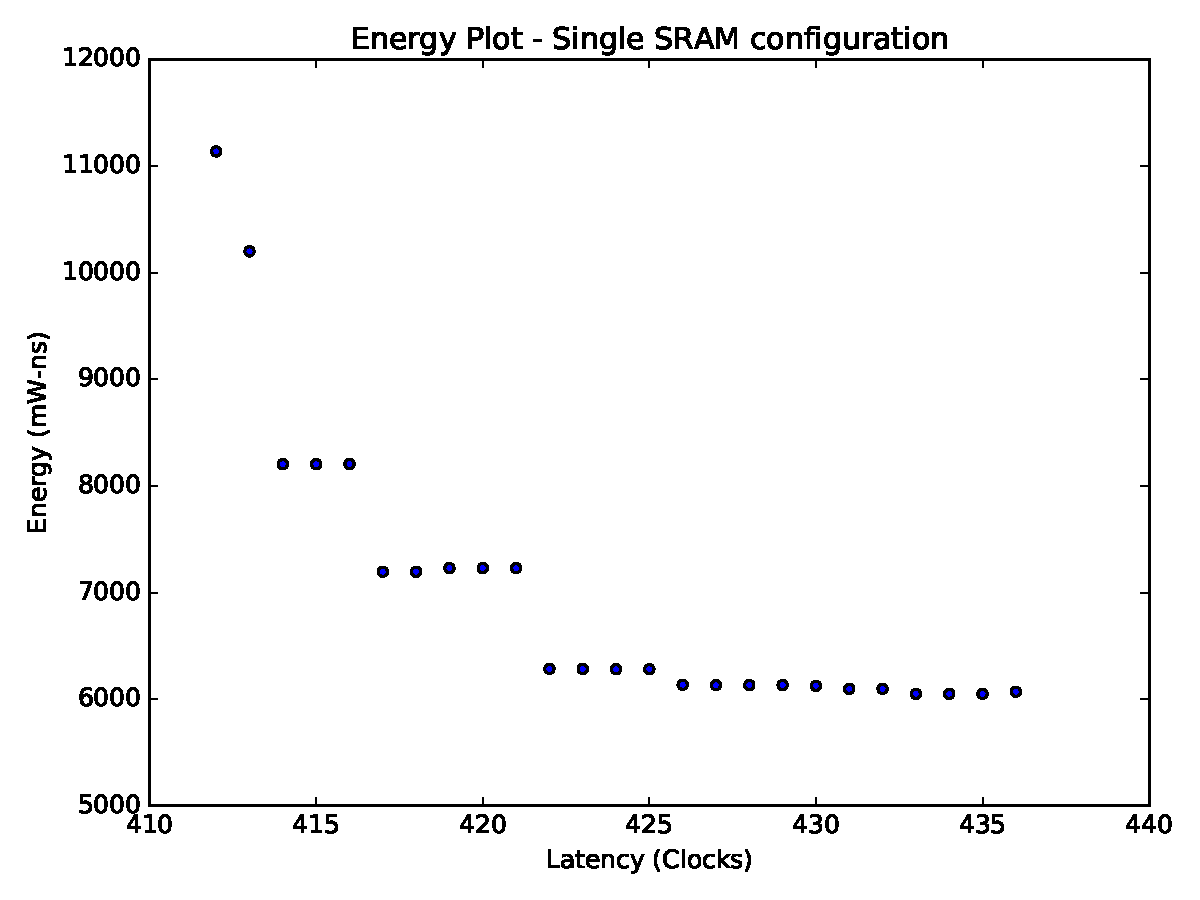
\includegraphics[width=\columnwidth]{graphs/energy_plot_single_sram.pdf}
\caption{\small Energy over Latency in clock cycles generated from a single configuration of a matrix vector multiplication of size 5x5. Each point corresponds to a generated hardware architecture. This configuration uses an SRAM Level 2 memory clocked at 350MHz, while the SRAM Level 1 memory and the Custom Processor are clocked at 1GHz.}
\label{fig:single_sram}
\end{figure}
In this experiment we used a 5x5 matrix vector multiplication as input application and we show the energy consumption of the hardware architectures generated by \frameworkname~from a single configuration. The configuration uses SRAM memories at all memory levels, the Level 2 memory is clocked at 350MHz, while the Level 1 and Custom Processor are clocked at 1GHz. Figure~\ref{fig:single_sram} shows the energy consumption and latency of the results. Each point represents a generated hardware architecture. The Maximum Parallel Architecture - starting point of our DSE - is the fastest architecture completing the computation in 412 clock cycles of the Custom Processor and it consumes $11.1^3$ mW-ns. The Most Sequential architecture - ending point of the DSE - is the slowest, compleating in 436 clock cycles and consuming $6^3$ mW-ns. Between these two extreme design points the DSE generates intermediate architectures offering various energy-latency tradeoffs. 


\subsection{MRAM vs SRAM layer 2 memory}

\begin{figure}[tb] 
\centering
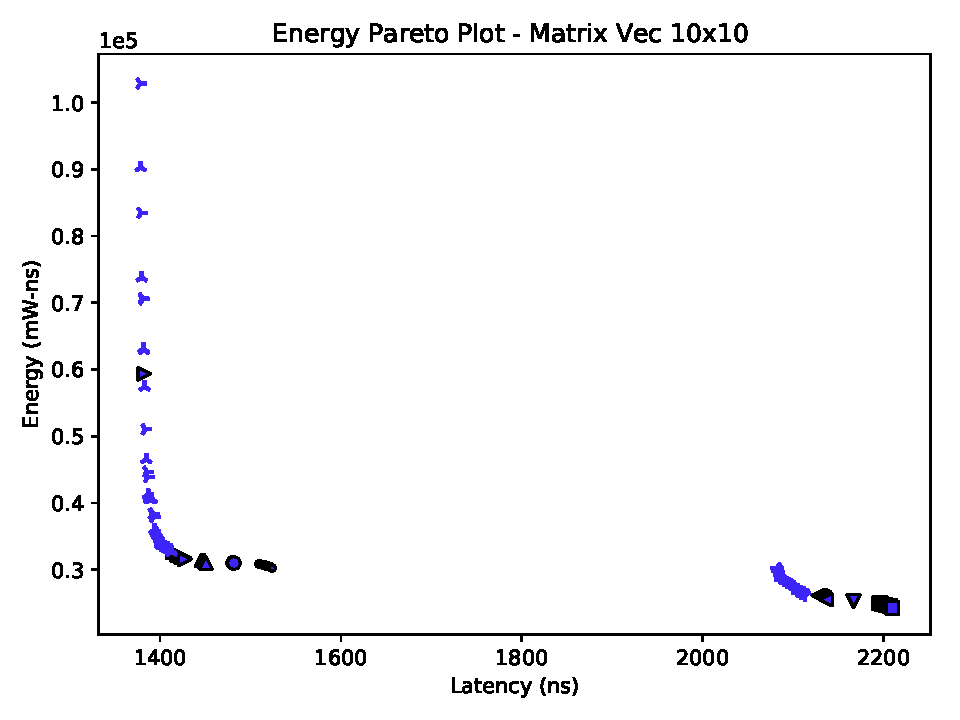
\includegraphics[width=\columnwidth]{graphs/EnergyParetoMatrixVec10.pdf}
    \caption{\small Energy Pareto optimal hardware architectures generated by \frameworkname~for a Matrix Vector multiplication 10x10, each point corresponds to an architecture generated by the framework.}
\label{fig:sram_vs_mram_pareto_vec}
\end{figure}

\begin{figure}[tb] 
\centering
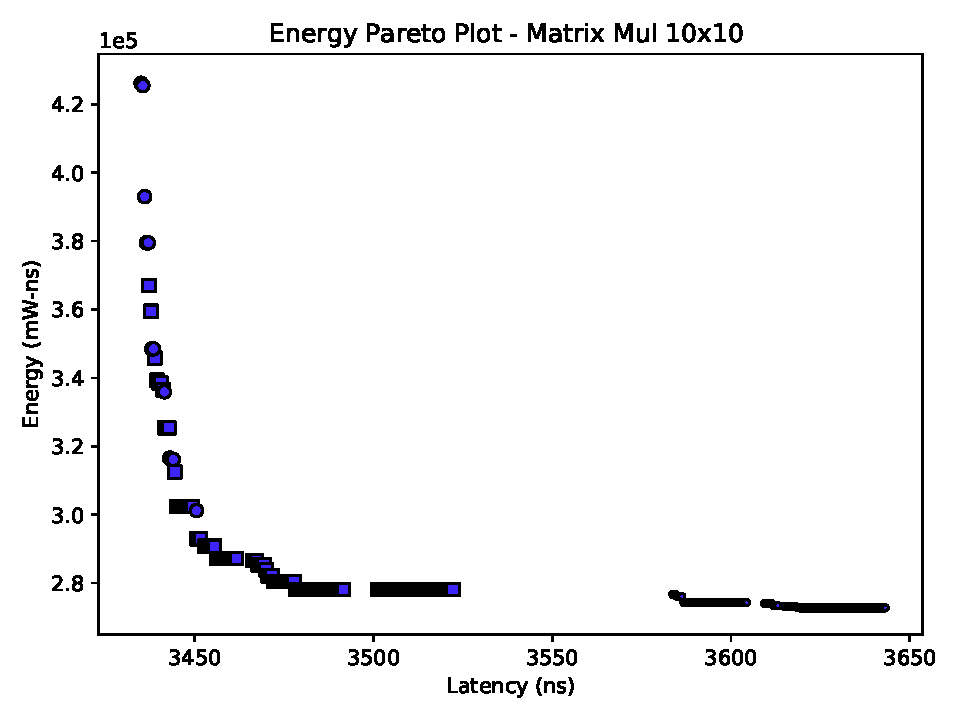
\includegraphics[width=\columnwidth]{graphs/EnergyParetoMatrixMul10.pdf}
    \caption{\small Energy Pareto optimal hardware architectures generated by \frameworkname~for a Matrix Vector multiplication 10x10, each point corresponds to an architecture generated by the framework.}
\label{fig:sram_vs_mram_pareto_mul}
\end{figure}
In this experiment we use \frameworkname~to compare two Level 2 MRAM memory against Level 2 SRAM memory. We used two input application a Matrix Vector 10x10, shown in Figure~\ref{fig:sram_vs_mram_pareto_vec} and a matrix multiply 10x10, in Figure~~\ref{fig:sram_vs_mram_pareto_mul}. Each point is relative to a hardware architecture generated by \frameworkname. The different shapes identify different input configurations: we compare two memory technologies at the Level 2 memory, MRAM and SRAM, clocked at 350MHz, while the SRAM Level 1 memory and the Custom Processor have clock frequencies ranging from 400MHz to 2GHz with steps of 200MHz. In both figures we can identify two clusters, one has higher energy consumption but lower latency, while the other has higher latency but lower latency consumption. These represent  configurations using respectively SRAM and MRAM technology at the Level 2 memory. In the case of the matrix vector application -Figure~\ref{fig:sram_vs_mram_pareto_vec} the fastest architecture - using SRAM memory - has a latency of 1375ns and consumes over $1^5$mW-ns. The most energy efficient SRAM architecture has instead a latency of 1525ns consuming under $0.3^5$mW-ns, begin 3x more energy efficient then the fastest with a 10\% increase in latency. The most energy efficient architecture using MRAM technology has instead a latency of 2210ns and consumes $0,24^5$mw-ns, hence having 45\% higher latency than the best SRAM counterpart, with 25\% decrease in power consumption. The matrix multiplication, Figure~\ref{fig:sram_vs_mram_pareto_mul}, performs 10 times more operation than the matrix vector multiplication, hence there is a clear overall increase in latency - about 30\% - and energy consumption - about 3x -  in comparison to the previous application. In this case the architecture using SRAM consuming the least amount of energy is has 2\% higher latency compared to the fastest one, but consumes 50\% less energy. However the introduction of MRAM technology in the Level 2 memory is not as beneficial as it was for the matrix vector application. The MRAM architecture consuming the least amount of energy has a 3\% slowdown compared to the most energy efficient SRAM, while attaining only a 2.2\% improvement in energy consumption. 

%\begin{itemize}
%	\item The most energy efficient designs are obtained using the highest possible clock for the Layer 2 SRAM memory (1GHz).
%	\item The architecture consuming less energy has a Layer 2 clock frequency of 1GHz and a Layer 1 clock frequency of 1600 MHz.
%\end{itemize}


\subsection{Different Matrix Vector Dimensions}
\begin{figure}[tb] 
\centering
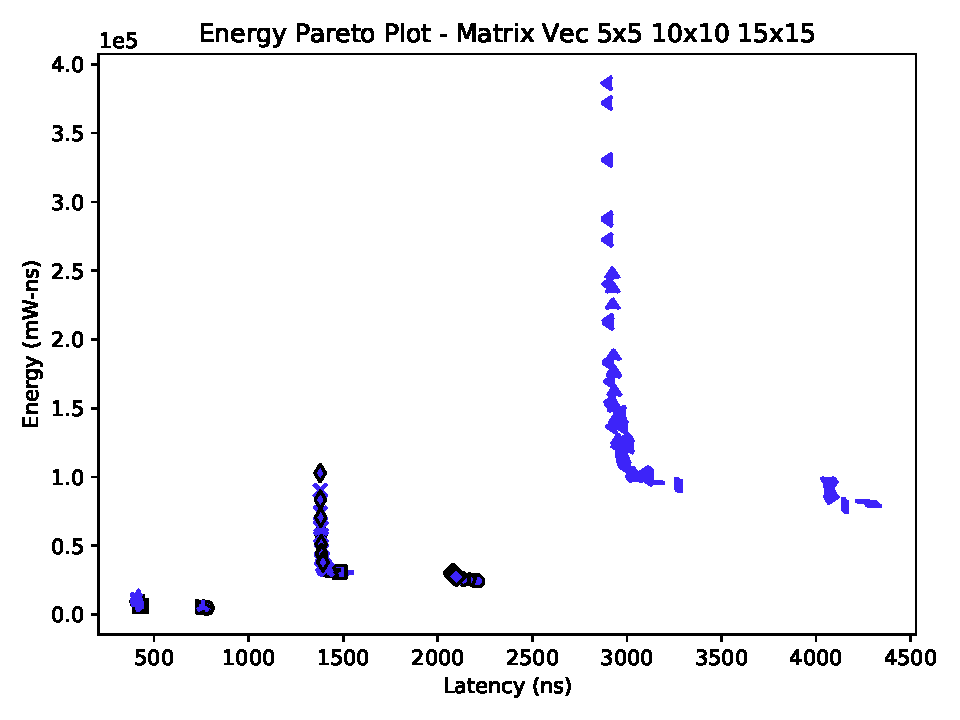
\includegraphics[width=\columnwidth]{graphs/EnergyParetoPlotMultipleSizeMAtrixVec.pdf}
    \caption{\small Energy Pareto optimal hardware architectures generated by \frameworkname for a Matrix Vector multiplication 10x10, each point corresponds to an architecture generated by the framework.}
\label{fig:sram_vs_mram_pareto_vec_sizes}
\end{figure}


